%
%  progress-presentation.tex
%  src
%
%  Created by Illya Starikov on 09/16/17.
%  Copyright 2017. Illya Starikov. All rights reserved.
%

% \documentclass[notes,xcolor=dvipsnames]{beamer}       % print frame + notes
% \documentclass[notes=only,xcolor=dvipsnames]{beamer}  % only notes
\documentclass[xclolor=dvipsnames]{beamer}            % only frames
%\documentclass[handout,xclolor=dvipsnames]{beamer}    % only frames, no pauses
\usepackage{soul,graphics}

\usetheme[logo=template-presentation/logo,faculty=ped]{fibeamer}

\usepackage{amssymb,amsmath,verbatim,graphicx,pdfpages,microtype,units,booktabs,upquote,xcolor,siunitx,csquotes,fancyvrb,newverbs,wrapfig,multicol,tikz,textcomp,wrapfig,cutwin}
\usepackage{fontawesome,setspace,rotchiffre,lipsum,listings,animate,listings}
\usepackage[xspace]{ellipsis}

\hypersetup{%
            colorlinks = true,
            linkcolor = orange,
            urlcolor  = orange,
            citecolor = orange,
            anchorcolor = orange}

\newcommand{\hugeslide}[1]{%
\begin{frame}[plain,c]
    \centering {\usebeamerfont*{frametitle} \usebeamercolor[fg]{frametitle}{\fontsize{40}{50}\selectfont\textit{#1}}}
\end{frame}
}

\newcommand{\presentaddcount}[1]{\addtocounter{#1}{1}\Roman{#1}}
\newcommand{\presentcount}[1]{\Roman{#1}}
\newcommand{\shellcmd}[1]{\texttt{\colorbox{gray!30}{#1}}}

\lstdefinelanguage{swift}
{%
  morekeywords={%
    func,if,then,else,for,in,while,do,switch,case,default,where,break,continue,fallthrough,return,
    typealias,struct,class,enum,protocol,var,func,let,get,set,willSet,didSet,inout,init,deinit,extension,
    subscript,prefix,operator,infix,postfix,precedence,associativity,left,right,none,convenience,dynamic,
    final,lazy,mutating,nonmutating,optional,override,required,static,unowned,safe,weak,internal,
    private,public,is,as,self,unsafe,dynamicType,true,false,nil,Type,Protocol,print
  },
  morecomment=[l]{//}, % l is for line comment
  morecomment=[s]{/*}{*/}, % s is for start and end delimiter
  morestring=[b]" % defines that strings are enclosed in double quotes
}

\definecolor{keyword}{HTML}{BA2CA3}
\definecolor{string}{HTML}{D12F1B}
\definecolor{comment}{HTML}{008400}
\definecolor{type}{HTML}{66B9AA}

\lstdefinestyle{Swift}{%
  language=swift,
  basicstyle=\ttfamily,
  showstringspaces=false, % lets spaces in strings appear as real spaces
  columns=fixed,
  keepspaces=true,
  keywordstyle=\color{keyword},
  stringstyle=\color{string},
  commentstyle=\color{comment},
  emph={Int,Character,Double,Float,Unsigned},
  emphstyle={\color{type}},
  morestring=[b]",
  escapeinside={(*}{*)}
}

\newcommand\syntaxbox[2][fill=orange!80]{%
    \tikz[baseline]\node[%
        inner ysep=0pt,
        inner xsep=2pt,
        anchor=text,
        rectangle,
        rounded corners=1mm,
        #1] {\strut#2};%
}


\title{UML Modeling (Presentation \#3)}
\subtitle{Special Topics (CS3001)}
\author{Illya Starikov}
\date{Sometimes In The Future}
\institute{Missouri University of Science and Technology}

\begin{document}
\begin{darkframes}
    \maketitle

    \begin{frame}
        \frametitle{A Brief Introduction}

        \begin{itemize}
            \item It's difficult to imagine a lot of objects interacting at the same time.
            \item It's also difficult for someone else to imagine these objects interacting when they have never seen them in use before.
            \item This where Uniform Modeling Language (UML) Diagramming comes in handy.
        \end{itemize}
    \end{frame}

    \begin{frame}
        \frametitle{A Brief Introduction}

        \begin{itemize}
            \item Uniform Modeling Language (UML) is a modeling language that helps visual a system, typically in programming.
            \item UML can be broken down into two simple interactions: Entities and Relationships.
                \begin{description}
                    \item[Entities] The actors in the system.
                    \item[Relationships] How actors interact with one another. These relationships can include: dependencies (A depends on B), generalization (A is a generalization of B), aggregation (A is an aggregation of B, C, D).
                \end{description}
        \end{itemize}
    \end{frame}

    \begin{frame}[fragile]
        \frametitle{A Brief Introduction}
        \begin{figure}[H]
            \centering
            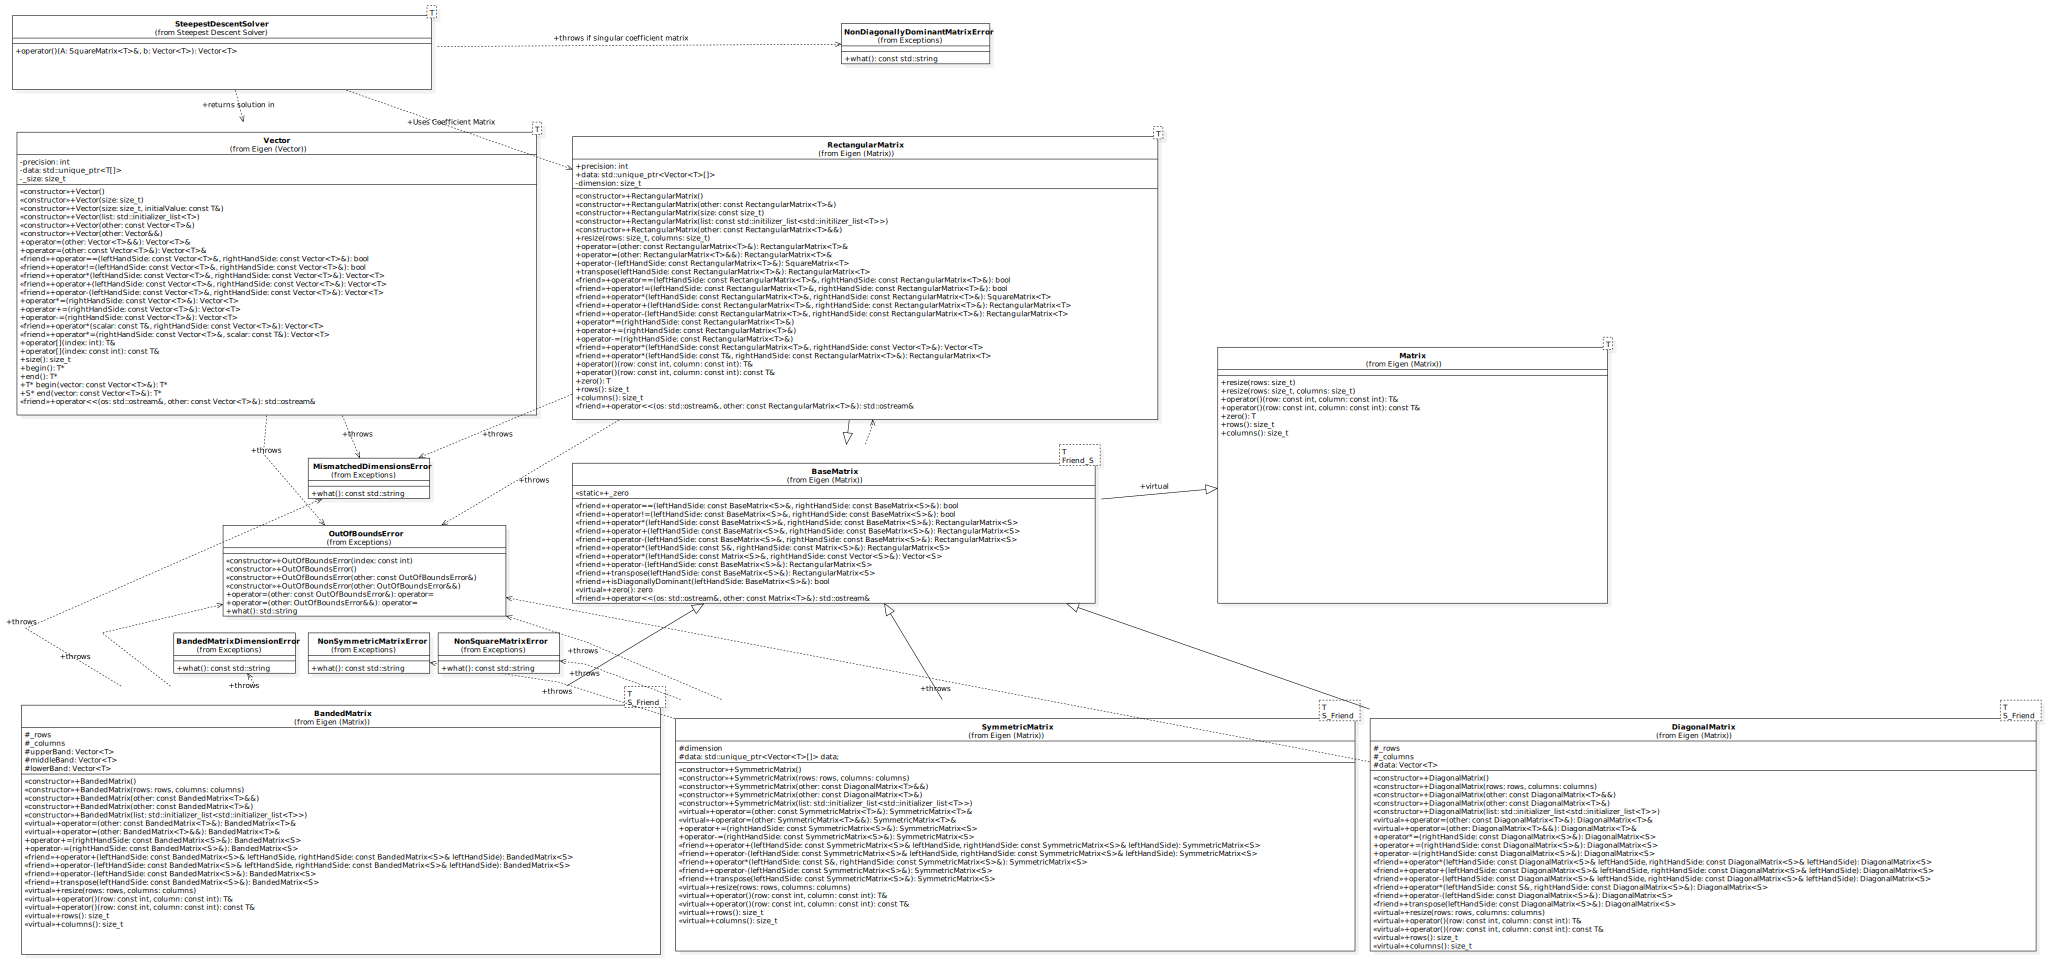
\includegraphics[width=\linewidth]{assets/uml.png}
            \caption{An example of a UML Diagram}
            \label{fig:sample-uml}
        \end{figure}
    \end{frame}


    \begin{frame}
        \frametitle{Prior Knowledge}

        \begin{itemize}
            \item I have had no prior experience with UML.
        \end{itemize}
    \end{frame}

    \begin{frame}
        \frametitle{Goals}

        \begin{itemize}
            \item To become fluent in UML Diagramming, with all associated entities and relationships.
            \item To become fluent in an application that is meant to do powerful UML diagramming.
        \end{itemize}
    \end{frame}

    \begin{frame}[fragile]
        \frametitle{StarUML}

        After a lot of searching, I settled on \href{http://staruml.io}{StarUML}. It was recommended all over the internet, and it seemed to be able to handle complicated diagrams.
    \end{frame}


    \begin{frame}[fragile]
        \frametitle{StarUML}
        \begin{figure}[H]
            \centering
            \includegraphics[width=\linewidth]{assets/staruml.png}
            \caption{An example of a UML Diagram}
            \label{fig:staruml}
        \end{figure}
    \end{frame}

    \begin{frame}
        \frametitle{Resources}

        \begin{itemize}
            \item Most of the learning came from playing around the tool. However, there were other resources I found to be useful.

            \item Online resources.
                \begin{itemize}
                    \item \href{http://staruml.io}{The official website.}
                    \item \href{http://staruml.io/extensions}{The extension gallery, to help automate the tedious parts.}
                    \item \href{https://holub.com/uml/}{A UML cheatsheet.}
                \end{itemize}

        \end{itemize}
    \end{frame}

    \begin{frame}
        \frametitle{Goal Accomplishment}

        \begin{itemize}
            \item Since the beginning of the semester, I have drastically become better at creating UML Diagrams. The evidence can be found with this presentation; \texttt{homework-2.png} was the first real UML Diagram I created, \texttt{homework-6.png} was the most recent one created.
        \end{itemize}
    \end{frame}

    \begin{frame}
        \frametitle{In Closing}

        All question, comments, and insults can be directed towards me:

        \begin{center}
            \begin{description}
                \item[\faComment] \href{mailto:starikov@mst.edu}{starikov@mst.com}
                \item[\faLinkedin] \href{https://www.linkedin.com/in/illyastarikov/}{Illya Starikov}
                \item[\faGithub] \href{https://github.com/IllyaStarikov/}{Illya Starikov}
                \item[\faRss] \href{https://freneticarray.com/}{FreneticArray.com}
            \end{description}
        \end{center}
    \end{frame}
\end{darkframes}
\end{document}
